\documentclass[12pt,a4paper]{article}
\usepackage[utf8]{inputenc}
\usepackage[T1]{fontenc}
\usepackage[T1]{fontenc}
\usepackage{amsmath,amssymb}
\usepackage{graphicx}
\usepackage{xcolor}
\usepackage{hyperref}
\usepackage{geometry}
\usepackage{tcolorbox}
\usepackage{needspace}
\usepackage{tikz}
\usepackage{titlesec}
\usepackage{array}
\usepackage{booktabs}
\usetikzlibrary{arrows.meta, positioning, shapes.geometric, calc}
\geometry{margin=2cm}

\definecolor{titrebleu}{RGB}{0,102,204}
\definecolor{defvert}{RGB}{0,153,76}
\definecolor{exempleorange}{RGB}{255,102,0}
\definecolor{algoviolet}{RGB}{153,0,153}
\definecolor{importantrouge}{RGB}{204,0,0}
\definecolor{fondgris}{RGB}{245,245,245}
\definecolor{fondjaune}{RGB}{255,250,205}
\definecolor{fondvert}{RGB}{230,255,230}
\definecolor{fondbleu}{RGB}{230,240,255}
\definecolor{fondrose}{RGB}{255,230,240}
\definecolor{fondorange}{RGB}{255,240,220}

\newtcolorbox{solution}{
    colback=fondvert, colframe=defvert,
    fonttitle=\bfseries, title=Solution, arc=3mm
}
\newtcolorbox{methode}{
    colback=fondbleu, colframe=titrebleu,
    fonttitle=\bfseries, title=Méthode, arc=3mm
}
\newtcolorbox{resultat}{
    colback=fondjaune, colframe=exempleorange,
    fonttitle=\bfseries, title=Résultat, arc=3mm
}
\newtcolorbox{remarque}{
    colback=fondrose, colframe=importantrouge,
    fonttitle=\bfseries, title=Remarque, arc=3mm
}
\newtcolorbox{etape}{
    colback=fondgris, colframe=algoviolet,
    fonttitle=\bfseries, arc=3mm
}

\titleformat{\section}
{\color{titrebleu}\normalfont\Large\bfseries}
{\color{titrebleu}\thesection}{1em}{}
\titleformat{\subsection}
{\color{defvert}\normalfont\large\bfseries}
{\color{defvert}\thesubsection}{1em}{}
\titleformat{\subsubsection}
{\color{algoviolet}\normalfont\normalsize\bfseries}
{\color{algoviolet}\thesubsubsection}{1em}{}

\title{
    \textbf{\Huge\color{titrebleu}Correction des Examens}\\[0.5em]
    \textbf{\Large\color{defvert}Réseaux et Optimisation --- Session 1}\\[0.5em]
    \large\color{algoviolet}N3 Informatique --- UCA
}
\author{Correction détaillée}
\date{}

\begin{document}

\maketitle
\tableofcontents
\newpage

%=================================================================
\part*{\color{titrebleu}EXAMEN A}
\addcontentsline{toc}{part}{Examen A}
%=================================================================

\section{Exercice 1 --- Graphe orienté $G_1$ (Figure 1)}

\textit{$G_1 = (V, E)$ avec $V = \{s,1,2,3,4,5,6\}$, orienté, poids sur les arcs incluant un arc négatif ($1 \to 4 : -3$).}

%---------------------------------------------------------------
\subsection{Question 1 : Représentation par niveaux (sans circuit)}

\begin{methode}
On construit les niveaux par induction : un sommet $v$ est au niveau $k$ si le plus long chemin depuis une source vers $v$ passe par $k$ arcs. Un nœud est \emph{source} s'il n'a aucun prédécesseur.
\end{methode}

\begin{solution}
\textbf{Analyse des prédécesseurs de chaque sommet :}
\begin{itemize}
    \item $s$ : aucun prédécesseur $\Rightarrow$ \textbf{Niveau 0}
    \item $1$ : seul prédécesseur $s$ (niveau 0) $\Rightarrow$ \textbf{Niveau 1}
    \item $2$ : seul prédécesseur $s$ (niveau 0) $\Rightarrow$ \textbf{Niveau 1}
    \item $4$ : prédécesseurs $1$ (niv.1) et $2$ (niv.1) $\Rightarrow$ \textbf{Niveau 2}
    \item $3$ : prédécesseurs $1$ (niv.1) et $4$ (niv.2) $\Rightarrow$ \textbf{Niveau 3}
    \item $5$ : prédécesseurs $2$ (niv.1) et $4$ (niv.2) $\Rightarrow$ \textbf{Niveau 3}
    \item $6$ : prédécesseurs $3$ (niv.3), $4$ (niv.2), $5$ (niv.3) $\Rightarrow$ \textbf{Niveau 4}
\end{itemize}

\medskip
\begin{center}
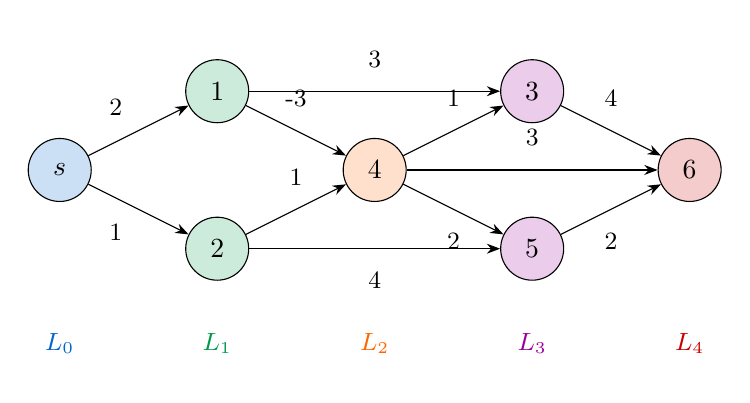
\begin{tikzpicture}[node distance=2.2cm, every node/.style={circle, draw, minimum size=8mm}]
    \node[fill=titrebleu!20] (s) at (0,0) {$s$};
    \node[fill=defvert!20] (1) at (2,1) {$1$};
    \node[fill=defvert!20] (2) at (2,-1) {$2$};
    \node[fill=exempleorange!20] (4) at (4,0) {$4$};
    \node[fill=algoviolet!20] (3) at (6,1) {$3$};
    \node[fill=algoviolet!20] (5) at (6,-1) {$5$};
    \node[fill=importantrouge!20] (6) at (8,0) {$6$};

    \draw[-{Stealth}] (s) -- node[above left,draw=none,fill=none]{\small 2} (1);
    \draw[-{Stealth}] (s) -- node[below left,draw=none,fill=none]{\small 1} (2);
    \draw[-{Stealth}] (1) -- node[above,draw=none,fill=none]{\small 3} (3);
    \draw[-{Stealth}] (1) -- node[above,draw=none,fill=none]{\small -3} (4);
    \draw[-{Stealth}] (2) -- node[above,draw=none,fill=none]{\small 1} (4);
    \draw[-{Stealth}] (2) -- node[below,draw=none,fill=none]{\small 4} (5);
    \draw[-{Stealth}] (4) -- node[above,draw=none,fill=none]{\small 1} (3);
    \draw[-{Stealth}] (4) -- node[below,draw=none,fill=none]{\small 2} (5);
    \draw[-{Stealth}] (4) -- node[above,draw=none,fill=none]{\small 3} (6);
    \draw[-{Stealth}] (3) -- node[above,draw=none,fill=none]{\small 4} (6);
    \draw[-{Stealth}] (5) -- node[below,draw=none,fill=none]{\small 2} (6);

    % Niveaux
    \node[draw=none,fill=none,color=titrebleu] at (0,-2.2) {\small $L_0$};
    \node[draw=none,fill=none,color=defvert] at (2,-2.2) {\small $L_1$};
    \node[draw=none,fill=none,color=exempleorange] at (4,-2.2) {\small $L_2$};
    \node[draw=none,fill=none,color=algoviolet] at (6,-2.2) {\small $L_3$};
    \node[draw=none,fill=none,color=importantrouge] at (8,-2.2) {\small $L_4$};
\end{tikzpicture}
\end{center}

Chaque sommet apparaît dans \textbf{un seul niveau} et tous les arcs vont d'un niveau vers un niveau strictement supérieur. Donc $G_1$ est \textcolor{importantrouge}{\textbf{sans circuit}}.
\end{solution}

%---------------------------------------------------------------
\subsection{Question 2 : Choix de l'algorithme}

\begin{solution}
Le graphe $G_1$ possède l'arc $1 \to 4$ de poids $-3$ (poids négatif).

\begin{itemize}
    \item \textcolor{importantrouge}{\textbf{Dijkstra :}} NON applicable --- requiert des poids non négatifs.
    \item \textbf{Bellman-Ford :} applicable (O($|V| \cdot |E|$)) mais pas optimal ici.
    \item \textcolor{defvert}{\textbf{Algorithme par niveaux (relaxation topologique) :}} MEILLEUR CHOIX --- $G_1$ est un graphe acyclique (DAG), donc on peut traiter les sommets en ordre topologique (ici par niveaux). Complexité : $O(|V| + |E|)$.
\end{itemize}

\textbf{Justification :} Puisque $G_1$ est sans circuit (DAG), on ne peut pas avoir de circuit absorbant. L'algorithme de relaxation par niveaux calcule les plus courts chemins en un seul passage en suivant l'ordre topologique.
\end{solution}

%---------------------------------------------------------------
\subsection{Question 3 : Plus courtes distances depuis $s$}

\begin{etape}{Exécution de l'algorithme par niveaux}
Initialisation : $d[s]=0$, $d[v]=+\infty$ pour tout $v \neq s$.

\medskip
\textbf{Niveau 0 --- traitement de $s$ :}
\[
d[1] = \min(+\infty,\ 0+2) = 2 \qquad d[2] = \min(+\infty,\ 0+1) = 1
\]

\textbf{Niveau 1 --- traitement de $1$ puis $2$ :}

Depuis $1$ ($d[1]=2$) :
\[
d[3] = \min(+\infty,\ 2+3) = 5 \qquad d[4] = \min(+\infty,\ 2+(-3)) = \mathbf{-1}
\]
Depuis $2$ ($d[2]=1$) :
\[
d[4] = \min(-1,\ 1+1) = -1 \text{ (inchangé)} \qquad d[5] = \min(+\infty,\ 1+4) = 5
\]

\textbf{Niveau 2 --- traitement de $4$ ($d[4]=-1$) :}
\[
d[3] = \min(5,\ -1+1) = \mathbf{0} \qquad d[5] = \min(5,\ -1+2) = \mathbf{1} \qquad d[6] = \min(+\infty,\ -1+3) = \mathbf{2}
\]

\textbf{Niveau 3 --- traitement de $3$ et $5$ :}

Depuis $3$ ($d[3]=0$) : $d[6] = \min(2,\ 0+4) = 2$ (inchangé)

Depuis $5$ ($d[5]=1$) : $d[6] = \min(2,\ 1+2) = 2$ (inchangé)
\end{etape}

\begin{resultat}
\[
\begin{array}{|c|c|c|c|c|c|c|}
\hline
\textbf{Sommet} & s & 1 & 2 & 3 & 4 & 5 \\\hline
d(\cdot) & 0 & 2 & 1 & 0 & -1 & 1 \\\hline
\end{array}
\qquad d(6) = 2
\]
\end{resultat}

%---------------------------------------------------------------
\subsection{Question 4 : Arborescence des plus courts chemins}

\begin{solution}
On détermine le prédécesseur $\pi[v]$ de chaque sommet :
\[
\pi[1]=s,\quad \pi[2]=s,\quad \pi[4]=1,\quad \pi[3]=4,\quad \pi[5]=4,\quad \pi[6]=4
\]

\begin{center}
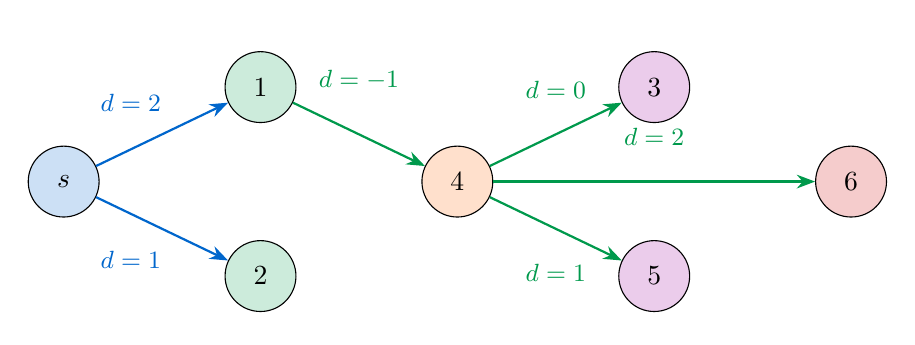
\begin{tikzpicture}[node distance=2.5cm, every node/.style={circle,draw,minimum size=9mm}]
    \node[fill=titrebleu!20] (s) at (0,0) {$s$};
    \node[fill=defvert!20] (1) at (2.5,1.2) {$1$};
    \node[fill=defvert!20] (2) at (2.5,-1.2) {$2$};
    \node[fill=exempleorange!20] (4) at (5,0) {$4$};
    \node[fill=algoviolet!20] (3) at (7.5,1.2) {$3$};
    \node[fill=algoviolet!20] (5) at (7.5,-1.2) {$5$};
    \node[fill=importantrouge!20] (6) at (10,0) {$6$};

    \draw[-{Stealth},thick,color=titrebleu] (s) -- node[above left,draw=none,fill=none]{\small $d=2$} (1);
    \draw[-{Stealth},thick,color=titrebleu] (s) -- node[below left,draw=none,fill=none]{\small $d=1$} (2);
    \draw[-{Stealth},thick,color=defvert] (1) -- node[above,draw=none,fill=none]{\small $d=-1$} (4);
    \draw[-{Stealth},thick,color=defvert] (4) -- node[above,draw=none,fill=none]{\small $d=0$} (3);
    \draw[-{Stealth},thick,color=defvert] (4) -- node[below,draw=none,fill=none]{\small $d=1$} (5);
    \draw[-{Stealth},thick,color=defvert] (4) -- node[above,draw=none,fill=none]{\small $d=2$} (6);
\end{tikzpicture}
\end{center}

\textbf{Chemins optimaux depuis $s$ :}
\[
s \xrightarrow{2} 1 \xrightarrow{-3} 4 \xrightarrow{1} 3 \quad (d=0),\qquad
s \xrightarrow{1} 2 \xrightarrow{\phantom{x}} \ldots \quad \text{(non utilisé pour les PCC vers 4,3,5,6)}
\]
\[
s \to 1 \to 4 \to 5 \quad (d=1), \qquad s \to 1 \to 4 \to 6 \quad (d=2)
\]
\end{solution}

\newpage
%=================================================================
\section{Exercice 2 --- Graphe $G_2$ (Figure 2) : Réseau sans fil}

\textit{$G_2$ : graphe non orienté, nœuds $\{a,b,c,d,e,f,g\}$, poids = énergie nécessaire. Arêtes : $a$-$e$:3, $a$-$c$:4, $c$-$g$:5, $e$-$f$:6, $f$-$g$:6, $c$-$d$:7, $a$-$b$:8, $b$-$c$:8, $b$-$d$:8, $c$-$e$:10, $c$-$f$:11, $d$-$g$:9.}

%---------------------------------------------------------------
\subsection{Questions 1--2 : Deux arbres couvrants d'énergie minimum}

\begin{methode}
Un arbre couvrant d'énergie minimum = arbre couvrant de poids minimum (MST). On utilise l'algorithme de Kruskal (trier les arêtes par poids croissant, ajouter une arête si elle ne crée pas de cycle).
\end{methode}

\begin{etape}{Algorithme de Kruskal --- Arêtes triées par poids}
$a$-$e$(3), $a$-$c$(4), $c$-$g$(5), $e$-$f$(6), $f$-$g$(6), $c$-$d$(7), $a$-$b$(8), $b$-$c$(8), $b$-$d$(8), $d$-$g$(9), $c$-$e$(10), $c$-$f$(11)

\begin{enumerate}
    \item $a$-$e$ (3) : ajouter $\to \{a,e\}$, $\{b\}$, $\{c\}$, $\{d\}$, $\{f\}$, $\{g\}$
    \item $a$-$c$ (4) : ajouter $\to \{a,c,e\}$
    \item $c$-$g$ (5) : ajouter $\to \{a,c,e,g\}$
    \item $e$-$f$ (6) : ajouter $\to \{a,c,e,f,g\}$
    \item $f$-$g$ (6) : $f$ et $g$ dans le même composant \textcolor{importantrouge}{\textbf{CYCLE}} $\to$ ignorer
    \item $c$-$d$ (7) : ajouter $\to \{a,c,d,e,f,g\}$
    \item Besoin de connecter $b$ : \textcolor{algoviolet}{\textbf{TROIS options de même poids 8 :}}
        \begin{itemize}
            \item $a$-$b$ (8) : $b \notin \{a,c,d,e,f,g\}$ $\to$ valide
            \item $b$-$c$ (8) : $b \notin \{a,c,d,e,f,g\}$ $\to$ valide
            \item $b$-$d$ (8) : $b \notin \{a,c,d,e,f,g\}$ $\to$ valide
        \end{itemize}
\end{enumerate}
\end{etape}

\begin{solution}
Les trois options donnent des MST \textbf{distincts mais de même coût} $= 3+4+5+6+7+8 = \mathbf{33}$ :

\medskip
\textbf{Arbre $T_1$} $=\{a$-$e(3),\ a$-$c(4),\ c$-$g(5),\ e$-$f(6),\ c$-$d(7),\ a$-$b(8)\}$\\
\textbf{Arbre $T_2$} $=\{a$-$e(3),\ a$-$c(4),\ c$-$g(5),\ e$-$f(6),\ c$-$d(7),\ b$-$c(8)\}$

\medskip
\textbf{Puissance de chaque nœud} $p(v)=$ poids maximal des arêtes incidentes à $v$ dans l'arbre :

\begin{center}
\begin{tabular}{|c|c|c|c|c|c|c|c||c|}
\hline
\textbf{Nœud} & $a$ & $b$ & $c$ & $d$ & $e$ & $f$ & $g$ & \textbf{Total} \\\hline
$p_{T_1}$ & $\max(8,4,3)=8$ & $8$ & $\max(4,5,7)=7$ & $7$ & $\max(3,6)=6$ & $6$ & $5$ & \textbf{47} \\\hline
$p_{T_2}$ & $\max(4,3)=4$ & $8$ & $\max(4,8,5,7)=8$ & $7$ & $\max(3,6)=6$ & $6$ & $5$ & \textbf{44} \\\hline
\end{tabular}
\end{center}

$T_2$ donne une \textbf{puissance totale plus faible} (44 vs 47), bien que les deux soient des MST.
\end{solution}

%---------------------------------------------------------------
\subsection{Question 3 : Algorithme BIP appliqué depuis $c$}

\begin{methode}
\textbf{BIP (Broadcast Incremental Power)} : à chaque étape, ajouter l'arête $(u,v)$ avec $u$ dans l'arbre, $v$ hors de l'arbre, qui minimise \textbf{le coût additionnel} $C(u,v) - p(u)$ (puissance supplémentaire nécessaire). Si $C(u,v) \le p(u)$, le coût additionnel est $0$.
\end{methode}

\begin{etape}{Exécution depuis $c$ ($p(c)=0$ initialement)}
\textbf{Étape 1} : Arêtes depuis $c$ : 
$c$-$a$(4), $c$-$g$(5), $c$-$d$(7), $c$-$e$(10), $c$-$f$(11). 
Minimum : $\mathbf{c}$-$\mathbf{a}(4)$, coût additionnel $=4-0=4$.
Ajouter $a$ : $p(c)=4$, $p(a)=4$.

\textbf{Étape 2} : Depuis $c$ ($p=4$) et $a$ ($p=4$) :
$c$-$g$(5)$: 5-4=1$, $c$-$d$(7)$: 3$, $a$-$e$(3)$: \max(3-4,0)=\mathbf{0}$, $a$-$b$(8)$: 4$.
Minimum : $\mathbf{a}$-$\mathbf{e}(3)$, coût $=0$ (car $p(a)=4 \ge 3$).
Ajouter $e$ : $p(a)=4$ (inchangé), $p(e)=3$.

\textbf{Étape 3} : Depuis $c$($p=4$), $a$($p=4$), $e$($p=3$) :
$c$-$g$(5)$: 1$, $c$-$d$(7)$: 3$, $a$-$b$(8)$: 4$, $e$-$f$(6)$: 6-3=3$.
Minimum : $\mathbf{c}$-$\mathbf{g}(5)$, coût $=1$.
Ajouter $g$ : $p(c)=5$, $p(g)=5$.

\textbf{Étape 4} : 
$c$-$d$(7)$: 7-5=2$, $a$-$b$(8)$: 4$, $e$-$f$(6)$: 3$.
Minimum : $\mathbf{c}$-$\mathbf{d}(7)$, coût $=2$.
Ajouter $d$ : $p(c)=7$, $p(d)=7$.

\textbf{Étape 5} :
$a$-$b$(8)$: 8-4=4$, $b$-$d$(8)$: 8-7=1$, $e$-$f$(6)$: 3$.
Minimum : $\mathbf{b}$-$\mathbf{d}(8)$, coût $=1$.
Ajouter $b$ : $p(d)=8$, $p(b)=8$.

\textbf{Étape 6} :
$e$-$f$(6)$: 3$.
Ajouter $\mathbf{e}$-$\mathbf{f}(6)$.
$p(e)=6$, $p(f)=6$.
\end{etape}

\begin{resultat}
\textbf{Arbre BIP} $= \{c$-$a(4),\ a$-$e(3),\ c$-$g(5),\ c$-$d(7),\ b$-$d(8),\ e$-$f(6)\}$

\begin{center}
\begin{tabular}{|c|c|c|c|c|c|c|c||c|}
\hline
\textbf{Nœud} & $a$ & $b$ & $c$ & $d$ & $e$ & $f$ & $g$ & \textbf{Total} \\\hline
$p_{\text{BIP}}$ & $4$ & $8$ & $7$ & $8$ & $6$ & $6$ & $5$ & $\mathbf{44}$ \\\hline
\end{tabular}
\end{center}
\end{resultat}

%---------------------------------------------------------------
\subsection{Question 4 : Borne sur la puissance totale minimum}

\begin{solution}
La puissance totale minimum $P^*$ du réseau vérifie :
\[
P^* \geq \max_{v \in V} p_{\min}(v)
\]
où $p_{\min}(v)$ est la puissance minimale imposée à $v$ par sa distance au voisin le plus éloigné dans tout arbre couvrant connexe.

\medskip
En comparant les résultats :
\begin{itemize}
    \item MST $T_1$ : puissance totale $= 47$
    \item MST $T_2$ : puissance totale $= 44$
    \item BIP depuis $c$ : puissance totale $= 44$
\end{itemize}

\textbf{Borne supérieure} sur $P^*$ : $P^* \leq 44$ (BIP et $T_2$ atteignent cette valeur).

\begin{remarque}
BIP ne garantit pas l'optimalité globale, mais donne souvent une meilleure solution que le MST seul. Ici, $P^*_{\min} \le 44$.
\end{remarque}
\end{solution}

\newpage
%=================================================================
\section{Exercice 3 --- Graphe $G_3$ (Figure 3) : Chemins arcs-disjoints et flot maximum}

\textit{$G_3$ : graphe orienté, source $s$, puits $t$. On rappelle : deux $st$-chemins sont arcs-disjoints s'ils n'ont aucun arc en commun.}

%---------------------------------------------------------------
\subsection{Question 1 : Définir les capacités}

\begin{solution}
Pour ramener la recherche du \textbf{nombre maximum de $st$-chemins arcs-disjoints} à un problème de \textbf{flot maximum} :

\textbf{Affecter la capacité $1$ à chaque arc} de $G_3$.

\textbf{Justification :} Un flot de valeur $k$ avec des capacités unitaires correspond exactement à $k$ chemins arcs-disjoints de $s$ à $t$ (chaque arc est utilisé au plus une fois). Par le théorème de décomposition en chemins, tout flot entier de valeur $k$ peut être décomposé en $k$ chemins $s$-$t$ arcs-disjoints.
\end{solution}

%---------------------------------------------------------------
\subsection{Question 2 : Déterminer le flot maximum}

\begin{etape}{Identification des chemins arcs-disjoints dans $G_3$}
On identifie les arcs de $G_3$ depuis les chemins visibles :
$s \to a,b,c,d$ ; $a \to i,f$ ; $b \to f$ ; $c \to f$ ; $d \to f$ ; $f \to h, g$ ; $g,h,i \to t$.

\medskip
\textbf{Recherche d'un flot maximum de valeur 3 (chemins arcs-disjoints) :}
\begin{itemize}
    \item $P_1$ : $s \to a \to i \to t$ \quad (arcs $sa$, $ai$, $it$)
    \item $P_2$ : $s \to b \to f \to h \to t$ \quad (arcs $sb$, $bf$, $fh$, $ht$)
    \item $P_3$ : $s \to c \to f \to g \to t$ \quad (arcs $sc$, $cf$, $fg$, $gt$)
\end{itemize}

\textbf{Vérification :} Ces 3 chemins utilisent 10 arcs \textbf{tous distincts} $\checkmark$

\medskip
\textbf{Peut-on atteindre 4 ?} Le 4\textsuperscript{e} chemin devrait utiliser $s \to d \to f$, mais tous les arcs sortants de $f$ ($fh$ et $fg$) sont déjà saturés dans $P_2$ et $P_3$. $\Rightarrow$ Le flot maximal est $\mathbf{3}$.
\end{etape}

\begin{resultat}
\[
\text{Nombre maximum de } st\text{-chemins arcs-disjoints} = f^* = \mathbf{3}
\]
\end{resultat}

%---------------------------------------------------------------
\subsection{Question 3 : Coupe minimum et interprétation}

\begin{solution}
\textbf{Coupe minimum} : $\{(i,t),\ (h,t),\ (g,t)\}$ --- les 3 arcs entrant dans $t$.

\[
\text{Capacité de la coupe} = 1 + 1 + 1 = 3 = f^*
\]

Ce qui confirme l'optimalité par le \textbf{théorème min-flot / max-coupe}.

\medskip
\textbf{Interprétation (Théorème de Menger)} : La coupe minimum $\{(i,t),(h,t),(g,t)\}$ représente un ensemble de 3 arcs dont la suppression déconnecte $s$ de $t$. Par le théorème de Menger (version arcs), le nombre maximum de $st$-chemins arcs-disjoints = capacité de la coupe minimum = \textbf{3}.

\begin{remarque}
En pratique : pour bloquer toute communication de $s$ à $t$ dans ce réseau, il suffit de couper les 3 arcs $\{(i,t),(h,t),(g,t)\}$ (les entrées du puits $t$). Il n'existe pas de coupe de capacité inférieure.
\end{remarque}
\end{solution}

\newpage
%=================================================================
\part*{\color{titrebleu}EXAMEN B}
\addcontentsline{toc}{part}{Examen B}
%=================================================================

\section{Exercice 1 --- Théorie et plus courts chemins}

%---------------------------------------------------------------
\subsection{Question 1.1 : Nombre de chemins élémentaires dans $G=(V,E)$}

\textit{$V=\{v_1,\ldots,v_n\}$, $E=\{(v_i,v_j) : 1 \le i < j \le n\}$ (tout arc va d'un indice plus petit vers un plus grand).}

\begin{solution}
Tout chemin élémentaire de $v_1$ à $v_n$ consiste à :
\begin{enumerate}
    \item Partir de $v_1$
    \item Choisir un \textbf{sous-ensemble} $S \subseteq \{v_2,\ldots,v_{n-1}\}$ de nœuds intermédiaires
    \item Les visiter en ordre croissant d'indice (imposé par la structure des arcs)
    \item Arriver à $v_n$
\end{enumerate}

Puisque pour tout $S$ il existe exactement un chemin (les nœuds doivent être visités en ordre croissant), le nombre de chemins élémentaires de $v_1$ à $v_n$ est :
\[
\boxed{2^{n-2}}
\]
(correspondant aux $2^{n-2}$ sous-ensembles possibles de $\{v_2,\ldots,v_{n-1}\}$).

\textbf{Exemple} : $n=4$, $V=\{v_1,v_2,v_3,v_4\}$. Chemins : $v_1 v_4$, $v_1 v_2 v_4$, $v_1 v_3 v_4$, $v_1 v_2 v_3 v_4$ $\Rightarrow$ $2^2=4$ chemins. $\checkmark$
\end{solution}

%---------------------------------------------------------------
\subsection{Question 1.2 : Algorithme pour $G_1$ (Figure 1, arc négatif $1\to 4 : -3$)}

\begin{solution}
\textbf{Choix : Algorithme de relaxation par ordre topologique (niveaux)} car $G_1$ est un DAG.

\textbf{Justification :}
\begin{itemize}
    \item $G_1$ contient l'arc $1 \to 4$ de poids $-3$ $\Rightarrow$ Dijkstra \textcolor{importantrouge}{\textbf{non applicable}}
    \item $G_1$ est sans circuit (voir Examen A, Exercice 1.1) $\Rightarrow$ pas de circuit absorbant
    \item Algorithme par niveaux : O($|V|+|E|$) $=$ O($n+m$), complexité optimale
\end{itemize}

\textbf{Résultat} (identique à l'Examen A, Ex 1.3) :
\[
d(s)=0,\ d(1)=2,\ d(2)=1,\ d(3)=0,\ d(4)=-1,\ d(5)=1,\ d(6)=2
\]
\textbf{Arborescence :} $s \!\to\! 1$, $s \!\to\! 2$, $1 \!\to\! 4$ ($d=-1$), $4 \!\to\! 3$ ($d=0$), $4 \!\to\! 5$ ($d=1$), $4 \!\to\! 6$ ($d=2$).
\end{solution}

%---------------------------------------------------------------
\subsection{Question 1.3 : Algorithme pour $G_2$ (Figure 2, poids non négatifs)}

\textit{$G_2$ : arcs $s\!\to\!1(1)$, $s\!\to\!2(2)$, $1\!\to\!3(2)$, $1\!\to\!2(1)$, $3\!\to\!4(0)$, $3\!\to\!6(3)$, $2\!\to\!4(1)$, $4\!\to\!5(2)$, $4\!\to\!6(4)$, $5\!\to\!4(1)$, $5\!\to\!6(5)$.}

\begin{solution}
\textbf{Choix : Algorithme de Dijkstra} car tous les poids sont $\ge 0$.
\end{solution}

\begin{etape}{Dijkstra depuis $s$ sur $G_2$}
\begin{center}
\renewcommand{\arraystretch}{1.2}
\begin{tabular}{|c|c|c|c|c|c|c|c|l|}
\hline
\textbf{Étape} & $s$ & $1$ & $2$ & $3$ & $4$ & $5$ & $6$ & \textbf{Extrait} \\\hline
Init & \textbf{0} & $\infty$ & $\infty$ & $\infty$ & $\infty$ & $\infty$ & $\infty$ & --- \\\hline
1 & 0 & \textbf{1} & 2 & $\infty$ & $\infty$ & $\infty$ & $\infty$ & $s$ (d=0) \\\hline
2 & 0 & 1 & \textbf{2} & 3 & $\infty$ & $\infty$ & $\infty$ & $1$ (d=1) \\\hline
3 & 0 & 1 & 2 & \textbf{3} & 3 & $\infty$ & $\infty$ & $2$ (d=2) \\\hline
4 & 0 & 1 & 2 & 3 & \textbf{3} & $\infty$ & 6 & $3$ (d=3) \\\hline
5 & 0 & 1 & 2 & 3 & 3 & \textbf{5} & 6 & $4$ (d=3) \\\hline
6 & 0 & 1 & 2 & 3 & 3 & 5 & \textbf{6} & $5$ (d=5) \\\hline
\end{tabular}
\end{center}
\end{etape}

\begin{resultat}
\[
d(s)=0,\quad d(1)=1,\quad d(2)=2,\quad d(3)=3,\quad d(4)=3,\quad d(5)=5,\quad d(6)=6
\]

\textbf{Arborescence :} $\pi[1]=s$, $\pi[2]=s$, $\pi[3]=1$, $\pi[4]=2$ (ou $3$, \emph{ex-æquo} : $s\!\to\!2\!\to\!4=3$ et $s\!\to\!1\!\to\!3\!\to\!4=3$), $\pi[5]=4$, $\pi[6]=3$.
\end{resultat}

\newpage
%=================================================================
\section{Exercice 2 --- Graphe $G_3$ (Figure 3) : Réseau sans fil, MST et BIP adapté}

\textit{$G_3$ non orienté, nœuds $\{1,\ldots,9\}$ : arêtes $3$-$5$(3), $1$-$3$(4), $1$-$2$(5), $3$-$4$(5), $2$-$5$(5), $5$-$6$(5), $2$-$4$(6), $7$-$8$(6), $7$-$9$(8), $8$-$9$(9), $6$-$7$(10).}

%---------------------------------------------------------------
\subsection{Question 1 : Arbre couvrant d'énergie minimum $T_1$}

\begin{etape}{Kruskal sur $G_3$}
Arêtes triées : $3$-$5$(3), $1$-$3$(4), $1$-$2$(5), $3$-$4$(5), $2$-$5$(5), $5$-$6$(5), $2$-$4$(6), $7$-$8$(6), $7$-$9$(8), $8$-$9$(9), $6$-$7$(10)

\begin{enumerate}
    \item $3$-$5$ (3) : ajouter $\to \{3,5\}$
    \item $1$-$3$ (4) : ajouter $\to \{1,3,5\}$
    \item $1$-$2$ (5) : ajouter $\to \{1,2,3,5\}$
    \item $3$-$4$ (5) : ajouter $\to \{1,2,3,4,5\}$
    \item $2$-$5$ (5) : cycle $\to$ ignorer
    \item $5$-$6$ (5) : ajouter $\to \{1,2,3,4,5,6\}$
    \item $2$-$4$ (6) : cycle $\to$ ignorer
    \item $7$-$8$ (6) : ajouter $\to \{7,8\}$
    \item $7$-$9$ (8) : ajouter $\to \{7,8,9\}$
    \item $8$-$9$ (9) : cycle $\to$ ignorer
    \item $6$-$7$ (10) : connecte $\{1,\ldots,6\}$ et $\{7,8,9\}$ $\to$ ajouter $\checkmark$
\end{enumerate}
\end{etape}

\begin{resultat}
$T_1 = \{3\text{-}5(3),\ 1\text{-}3(4),\ 1\text{-}2(5),\ 3\text{-}4(5),\ 5\text{-}6(5),\ 7\text{-}8(6),\ 7\text{-}9(8),\ 6\text{-}7(10)\}$

Coût total $= 3+4+5+5+5+6+8+10 = \mathbf{46}$
\end{resultat}

%---------------------------------------------------------------
\subsection{Question 2 : Puissance de chaque nœud sur $T_1$}

\begin{solution}
La puissance $p(v)=$ poids maximal des arêtes incidentes à $v$ dans $T_1$ :

\begin{center}
\begin{tabular}{|c|c|l|c|}
\hline
\textbf{Nœud} & \textbf{Arêtes incidentes dans $T_1$} & \textbf{Calcul} & $p(v)$ \\\hline
1 & $1$-$3$(4), $1$-$2$(5) & $\max(4,5)$ & \textbf{5} \\\hline
2 & $1$-$2$(5) & $\max(5)$ & \textbf{5} \\\hline
3 & $3$-$5$(3), $1$-$3$(4), $3$-$4$(5) & $\max(3,4,5)$ & \textbf{5} \\\hline
4 & $3$-$4$(5) & $\max(5)$ & \textbf{5} \\\hline
5 & $3$-$5$(3), $5$-$6$(5) & $\max(3,5)$ & \textbf{5} \\\hline
6 & $5$-$6$(5), $6$-$7$(10) & $\max(5,10)$ & \textbf{10} \\\hline
7 & $6$-$7$(10), $7$-$8$(6), $7$-$9$(8) & $\max(10,6,8)$ & \textbf{10} \\\hline
8 & $7$-$8$(6) & $\max(6)$ & \textbf{6} \\\hline
9 & $7$-$9$(8) & $\max(8)$ & \textbf{8} \\\hline\hline
\multicolumn{3}{|r|}{\textbf{Puissance totale}} & \textbf{59} \\\hline
\end{tabular}
\end{center}
\end{solution}

%---------------------------------------------------------------
\subsection{Question 3 : Algorithme BIP adapté sur $G_3$}

\begin{methode}
\textbf{BIP adapté} : à chaque étape, ajouter l'arête $(u,v)$ ($u \in$ arbre, $v \notin$ arbre) minimisant
\[
a(u) + a(v) \quad \text{avec} \quad a(u) = \max\bigl(C(u,v) - p(u),\ 0\bigr)
\]
Début depuis le nœud 1.
\end{methode}

\begin{etape}{Exécution du BIP adapté depuis le nœud 1}
\textbf{Étape 1} : $p(1)=0$. Arêtes de 1 : $1$-$3$(4), $1$-$2$(5).
Coûts : $a(1)+a(3)=4+4=8$ ; $a(1)+a(2)=5+5=10$. Min : $\mathbf{1}$-$\mathbf{3}(4)$. $p(1)=4$, $p(3)=4$.

\textbf{Étape 2} : Depuis 1($p=4$), 3($p=4$). 
$1$-$2$(5)$: 1+5=6$, $3$-$5$(3)$: \max(3-4,0)+3=0+3=\mathbf{3}$, $3$-$4$(5)$: 1+5=6$.
Min : $\mathbf{3}$-$\mathbf{5}(3)$. $p(3)$ inchangé, $p(5)=3$.

\textbf{Étape 3} : Depuis 1($p=4$), 3($p=4$), 5($p=3$).
$1$-$2$(5)$: 1+5=6$, $3$-$4$(5)$: 1+5=6$, $5$-$2$(5)$: 2+5=7$, $5$-$6$(5)$: 2+5=7$.
Min ($ex$-$\ae{}quo$) : $\mathbf{1}$-$\mathbf{2}$ ou $\mathbf{3}$-$\mathbf{4}(5)$. Choisir $1$-$2$. $p(1)=5$, $p(2)=5$.

\textbf{Étape 4} : Depuis 1($p=5$), 3($p=4$), 5($p=3$), 2($p=5$).
$3$-$4$(5)$: 1+5=6$, $2$-$4$(6)$: 1+6=7$, $5$-$6$(5)$: 2+5=7$.
Min : $\mathbf{3}$-$\mathbf{4}(5)$. $p(3)=5$, $p(4)=5$.

\textbf{Étape 5} : Depuis 1($p=5$), 3($p=5$), 5($p=3$), 2($p=5$), 4($p=5$).
$5$-$6$(5): $2+5=7$, $2$-$4$(6): cycle.
Min : $\mathbf{5}$-$\mathbf{6}(5)$. $p(5)=5$, $p(6)=5$.

\textbf{Étape 6} : Depuis 6($p=5$): $6$-$7$(10)$: 5+10=15$. Ajouter $\mathbf{6}$-$\mathbf{7}(10)$. $p(6)=10$, $p(7)=10$.

\textbf{Étape 7} : Depuis 7($p=10$): $7$-$8$(6)$: 0+6=6$, $7$-$9$(8)$: 0+8=8$.
Min : $\mathbf{7}$-$\mathbf{8}(6)$. $p(7)$ inchangé, $p(8)=6$.

\textbf{Étape 8} : $7$-$9$(8)$: 0+8=8$, $8$-$9$(9)$: 3+9=12$.
Ajouter $\mathbf{7}$-$\mathbf{9}(8)$. $p(9)=8$.
\end{etape}

\begin{resultat}
\textbf{Arbre BIP adapté} $= \{1\text{-}3(4),\ 3\text{-}5(3),\ 1\text{-}2(5),\ 3\text{-}4(5),\ 5\text{-}6(5),\ 6\text{-}7(10),\ 7\text{-}8(6),\ 7\text{-}9(8)\}$

\textbf{Puissances :} $p(1)=5$, $p(2)=5$, $p(3)=5$, $p(4)=5$, $p(5)=5$, $p(6)=10$, $p(7)=10$, $p(8)=6$, $p(9)=8$

\textbf{Puissance totale BIP adapté} $= 5+5+5+5+5+10+10+6+8 = \mathbf{59}$
\end{resultat}

\begin{remarque}
Ici le BIP adapté converge vers le \textbf{même arbre que le MST} $T_1$. La puissance totale de 59 est dominée par l'arête $6$-$7$(10) indispensable pour connecter les deux clusters du réseau.
\end{remarque}

%---------------------------------------------------------------
\subsection{Question 4 : Borne sur la puissance totale minimum}

\begin{solution}
La puissance minimale du nœud 7 est forcément $\ge 10$ (car l'arête $6$-$7$ de poids 10 est un pont : toute arborescence connexe doit l'inclure ou une arête de poids $\ge 10$ pour connecter les clusters $\{1\ldots6\}$ et $\{7,8,9\}$).

Donc $P^* \ge p(6) + p(7) \ge 10 + 10 = 20$ (contribution des deux extrémités du pont).

Borne inférieure sur la puissance totale : $P^* \ge 59$ dans ce cas (le graphe est rigide sur le pont $6$-$7$).
\end{solution}

\newpage
%=================================================================
\section{Exercice 3 --- Graphe $G_4$ (Figure 4) : Flot maximum avec valeurs $a/b$}

%---------------------------------------------------------------
\subsection{Question 1 : Déterminer le flot maximum depuis $s$ vers $p$}

\begin{methode}
Avec les valeurs $a/b$ (flot courant / capacité) sur chaque arc :
\begin{enumerate}
    \item Calculer la valeur du flot actuel : $f_0 = \sum_{(s,v) \in E} a(s,v)$
    \item Construire le \textbf{graphe résiduel} $G^r$ : pour chaque arc $(u,v)$, 
        \begin{itemize}
            \item Arc avant $(u,v)$ de capacité résiduelle $b(u,v) - a(u,v)$
            \item Arc arrière $(v,u)$ de capacité résiduelle $a(u,v)$
        \end{itemize}
    \item Chercher un chemin augmentant de $s$ à $p$ dans $G^r$ (BFS ou DFS)
    \item Si aucun chemin augmentant $\to$ flot actuel est maximum
\end{enumerate}
\end{methode}

\begin{solution}
\textbf{Note :} Lire les valeurs $a/b$ depuis la Figure 4. Pour chaque arc, vérifier si la capacité résiduelle permet une augmentation. Si le flot $a$ est déjà maximum, la coupe minimale confirme l'optimalité.

\textbf{Condition d'optimalité :} Un flot $f$ est maximum si et seulement si il n'existe pas de chemin augmentant dans le graphe résiduel (théorème de Ford-Fulkerson).
\end{solution}

%---------------------------------------------------------------
\subsection{Question 2 : Capacité sur le nœud 3 (capacité $= 4$)}

\begin{solution}
\textbf{Signification} : Le sommet 3 ne peut transmettre qu'un flot de $\le 4$ unités en tout (capacité nodale).

\textbf{Technique de dédoublement de nœud} : Remplacer le nœud $3$ par deux nœuds $3_{in}$ et $3_{out}$ reliés par un arc $(3_{in}, 3_{out})$ de capacité $4$ :
\begin{itemize}
    \item Tous les arcs \emph{entrant} en 3 arrivent à $3_{in}$
    \item Tous les arcs \emph{sortant} de 3 partent de $3_{out}$
    \item L'arc $3_{in} \to 3_{out}$ a capacité $\min(4,\ \text{flot passant par 3})$
\end{itemize}

\textbf{Impact} : Si le flot optimal passant par 3 dans la question précédente était $\le 4$, alors \textbf{le flot maximum ne change pas}. Si le flot passait par 3 avec plus de 4 unités, il faudrait recalculer en tenant compte de cette contrainte.
\end{solution}

\newpage
%=================================================================
\section{Exercice 4 --- Stations radio (Dominant connexe)}

%---------------------------------------------------------------
\subsection{Question 1 : Problème évoqué}

\begin{solution}
Cette situation correspond au problème de \textbf{l'ensemble dominant de cardinalité minimum} (\textit{Minimum Dominating Set}).

Un ensemble $D \subseteq V$ est \textbf{dominant} si tout village $v \notin D$ est à distance $\le 50$ km d'au moins un village de $D$. Un village avec station couvre lui-même et tous ses voisins dans le graphe réduit $G_5^1$.

\textbf{Complexité} : Ce problème est NP-difficile en général, mais des heuristiques greedy (gloutonnes) donnent une approximation en $O(\ln \Delta)$ du minimum.
\end{solution}

%---------------------------------------------------------------
\subsection{Question 2 : Graphe $G_5^1$ et placement des stations (rayon 50 km)}

\begin{solution}
\textbf{(a) Extraction de $G_5^1$} : 
Garder uniquement les arêtes de $G_5$ (distances inter-villages) de poids $\le 50$ km. Toute arête de poids $> 50$ km est supprimée.

\textbf{(b) Placement optimal} : Appliquer l'heuristique gloutonne :
\begin{enumerate}
    \item Tant qu'il existe des villages non couverts :
    \item Choisir le village qui couvre le maximum de villages non encore couverts
    \item L'ajouter à $D$ (lui attribuer une station radio)
\end{enumerate}

\begin{remarque}
Appliquer cette méthode au graphe $G_5^1$ spécifique donné dans la Figure 5 (non visible ici). Le résultat est un ensemble dominant $D$ de taille minimale ou proche du minimum.
\end{remarque}
\end{solution}

%---------------------------------------------------------------
\subsection{Question 3 : Rayon étendu à 70 km}

\begin{solution}
Avec un rayon de 70 km, le graphe $G_5^{1'}$ est obtenu en gardant les arêtes de $G_5$ de poids $\le 70$ km. Ce graphe a \textbf{plus d'arêtes} que $G_5^1$.

\textbf{Conséquence} : Chaque station couvre un rayon plus grand $\Rightarrow$ l'ensemble dominant minimum $D'$ peut avoir \textbf{moins de stations} que $D$.

Si certains arcs entre 51 et 70 km deviennent actifs, des villages précédemment isolés peuvent être couverts par une station existante, réduisant le nombre de stations nécessaires.

\textbf{Méthode} : Reconstruire $G_5^{1'}$, puis appliquer la même heuristique pour trouver le nouvel ensemble dominant minimum $D'$.
\end{solution}

%=================================================================
\newpage
\section*{\color{titrebleu}Synthèse des résultats clés}
\addcontentsline{toc}{section}{Synthèse}

\begin{center}
\renewcommand{\arraystretch}{1.4}
\begin{tabular}{|p{3.5cm}|p{4cm}|p{6.5cm}|}
\hline
\textbf{Problème} & \textbf{Résultat} & \textbf{Algorithme} \\\hline
PCC sur DAG avec arc $-3$ & $d(6)=2$, $d(4)=-1$ & Relaxation topologique O($V+E$) \\\hline
PCC sur graphe $\ge 0$ ($G_2$) & $d(6)=6$, $d(4)=3$ & Dijkstra O($V^2$) \\\hline
MST de $G_2$ (a-g) & Coût = 33, 3 MSTs possibles & Kruskal \\\hline
Puissance totale MST / BIP & 47 / 44 (gain de BIP) & BIP commence depuis $c$ \\\hline
Chemins arcs-disjoints $G_3$ & Max = 3 chemins & Flot max, capacités unitaires \\\hline
Coupe min $G_3$ & $\{(i,t),(h,t),(g,t)\}$, val=3 & Menger : flot max = coupe min \\\hline
Chemins $v_1 \to v_n$ dans DAG complet & $2^{n-2}$ & Dénombrement par sous-ensembles \\\hline
MST de $G_3$ (1-9) & Coût = 46 & Kruskal \\\hline
Dominant pour stations radio & Voir $G_5^1$, $G_5^{1'}$ & Heuristique gloutonne \\\hline
\end{tabular}
\end{center}

\vspace{2em}
\begin{center}
\textcolor{titrebleu}{\rule{0.6\textwidth}{1.5pt}}\\[0.5em]
\textit{\large Bon courage pour l'examen !}\\[0.3em]
\textcolor{defvert}{\small Optimisation dans les Réseaux --- Bendali-Mailfert}
\end{center}

\end{document}
